\documentclass[12pt,a4paper,UTF8]{article}
% \usepackage{ctex} % Chinese support
\usepackage{graphicx} % Insert images
\usepackage{listings} % Print source code
\usepackage{color} % Color support
\usepackage{booktabs} % Professional table support
\usepackage{pdflscape} % Landscape pages support in PDF
\usepackage{hyperref} % Hypertext links support for cross-referencing

% Customize hyperref format (it's set to no special format here)
\hypersetup{hidelinks}

% Declare directories to search for graphics files for graphicx
\graphicspath{{figures/}{logo/}}

% Define source code style for listings
\lstdefinestyle{python}{
  language=Python,
  basicstyle=\ttfamily\footnotesize,
  keywordstyle=\bfseries\color[rgb]{0, 0, 1},
  identifierstyle=\color[rgb]{0.5, 0.3, 0.1},
  stringstyle=\color[rgb]{0.6, 0.1, 0.1},
  commentstyle=\itshape\color[rgb]{0.05, 0.5, 0.05},
  backgroundcolor=\color[gray]{0.95},
  numbers=left,
  numbersep=5pt,
  numberstyle=\color[gray]{0.6},
  breaklines=true
}

% Define new command for title page
\newcommand{\reporttitle}[2]{
  \LARGE\textsf{#1}\quad\underline{\makebox[12em]{#2}}
}
\newcommand{\reportinfo}[2]{
  \large\makebox[4em]{\textsf{#1}}\quad\underline{\makebox[18em]{#2}}
}

% The document begins here
\begin{document}
\begin{titlepage}
  \centering
  \vspace*{\fill}
  
\includegraphics[height=144pt]{nju-logo}\\[48pt]
  {\huge\textsf{Lab Report}}\\[48pt]
  \reporttitle{Lab Name}{Forwarding \& ARP Request}\\[72pt]

  \reportinfo{Course}{Computer Network}\\[8pt]
  \reportinfo{Major}{Computer Science and Technology}\\[8pt]
  \reportinfo{Id}{191220129}\\[8pt]
  \reportinfo{Name}{Shangyu.Xing}\\[8pt]
  \reportinfo{Email}{191220129@smail.nju.edu.cn}\\[8pt]
  \reportinfo{Date}{2021.04}\\
  \vspace*{\fill}
\end{titlepage}

\tableofcontents
\newpage

\section{Objective}
\begin{itemize}
	\item Learn address resolution protocol and how to implement it;
	\item learn forwarding rules of a layer-3 router;
	\item learn to implement hardware logic using the Switchyard framework;
	\item learn to capture network package using wireshark.
\end{itemize}

\section{Requirements}
This lab requires to implement a router who can forward packets according to preset rules and send ARP requests when necessary.
\begin{itemize}
	\item Implement a forwarding table;
	\item handle ARP request;
	\item try out multithreading.
\end{itemize}

\section{Procedure}
I completed all the tasks as required, \textbf{using multithreading as implementation}.
In this section, I will explain how I did my work in detail.

\subsection{Implement Forwarding Table}
To build the forwarding table, I need to complete the following steps:
\begin{enumerate}
	\item initialize the table according to interfaces on the router;
	\item append the file content to it.
\end{enumerate}
I used a list to store data. Every entry in the list consists 3 pieces -- [prefix to match: IPv4Network, next hop address: IPv4Address, interface: str].
Note that after initialization the table must be sorted according to length of netmask (descending), since the match order is from head to tail.
\lstinputlisting[style=python]{1.py}
Besides, to facilitate querying, I added a query method. It returns next hop address and interface when queried with an IP address.
\lstinputlisting[style=python]{2.py}

\subsection{Send ARP Request and Forward Packet}
\subsubsection{Forwarding Logic}
A router should do the following to forward a packet:
\begin{enumerate}
	\item decrease its ttl field in Network header;
	\item query the forwarding table or send arp request for next hop address and interface;
	\item query the arp table for mac address of the next hop ip;
	\item modify src and dst field in the ethernet header and send it out of the interface.
\end{enumerate}
\lstinputlisting[style=python]{3.py}

\subsubsection{ARP Request and Reply Handling}
To maintain a queue containing packets waiting for arp reply, we should create a python class for it. The class consists of a list containing waiting packets and other related data. It has the following methods:
\begin{itemize}
	\item \textbf{send\_arp\_request} -- send request and update timestamp and retry times
	\lstinputlisting[style=python]{4.py}
	\item \textbf{insert} -- insert a packet waiting for reply
	\lstinputlisting[style=python]{5.py}
	\item \textbf{release} -- modify and send out blocked packets once receiving an arp reply
	\lstinputlisting[style=python]{6.py}
	\item \textbf{check\_timeout} -- check all entries in table and resend request if it timeout
	\lstinputlisting[style=python]{7.py}
\end{itemize}
Note that when an entry timeout, it is not physically deleted; instead it is marked invalid, hiding from querying or printing. \\

\subsection{Multithreading}
It is natural to implement another thread to maintain the queue and send arp request, while the main thread only handle received packets. If an arp reply is received, the main thread sends arp thread a signal noticing that an entry in table should be removed. Note that arp thread will terminate when main thread exits, so its property 'daemon' should be set to true. \\
The behavior of arp thread is very simple; it only repeatedly calls the method check\_timeout of ArpQueue every 0.1s.
\lstinputlisting[style=python]{8.py}

\section{Result}
\subsection{Testcase}
Firstly I tested my code with switchyard testcases:
\begin{figure}[htbp]
	\centering
	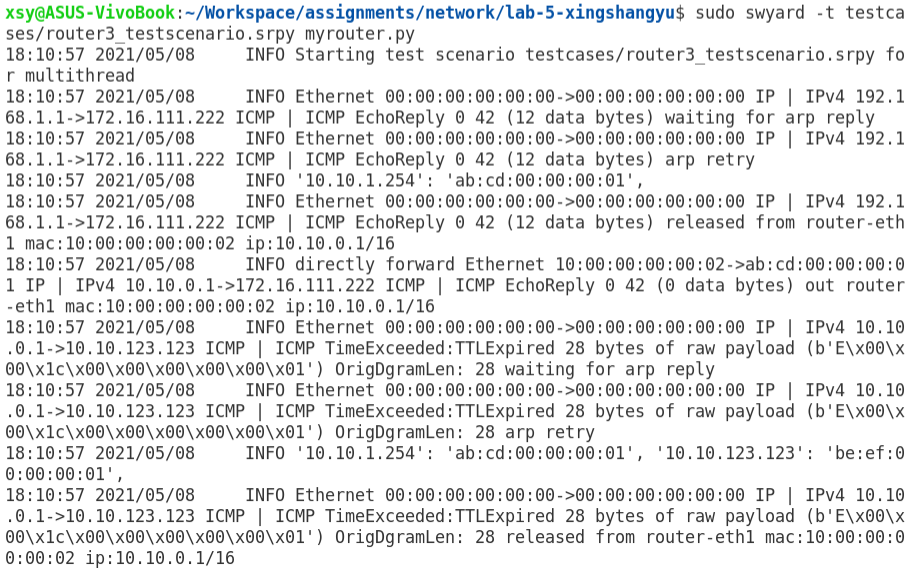
\includegraphics[width=\textwidth]{1}
	\caption{Switchyard test result}
\end{figure}
\newpage
It seems that switchyard testing framework works well with multithreading!

\subsection{Deployment}
To perform a test in mininet, I commanded server1 to ping client 2 times and ran wireshark on router's interface eth-2. I got a result of 0\% drop and this record:
\begin{figure}[htbp]
	\centering
	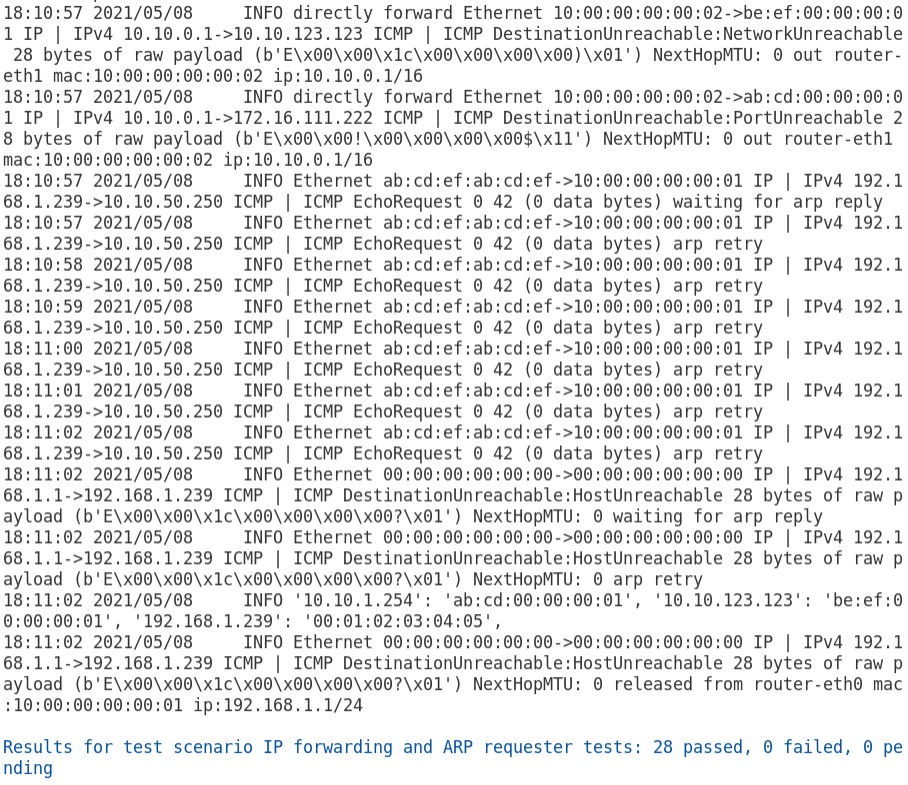
\includegraphics[width=\textwidth]{2}
	\caption{Wireshark capture result}
\end{figure}
\begin{figure}[htbp]
	\centering
	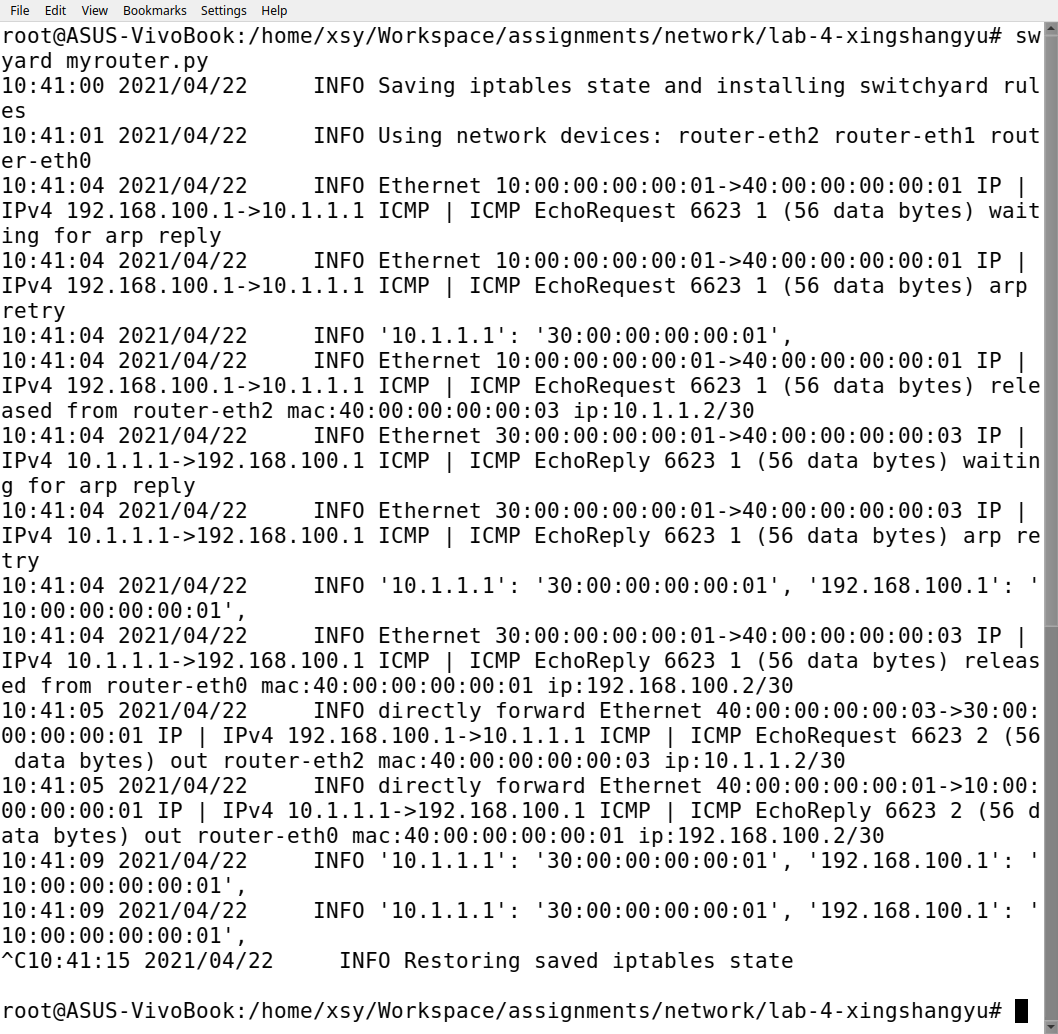
\includegraphics[width=\textwidth]{3}
	\caption{Router's log}
\end{figure}
\newpage
What happened in the network was this:
\begin{enumerate}
	\item server1 broadcast arp packet, and the router found that it was directed at it;
	\item The router made an arp response to server1 and cached server1's (ip, mac) pair in its arp table;
	\item server1 extract mac from the response, then sent echo requests packet to the router;
	\item the router looked for its forwarding table and got next hop address, but it didn't konw the mac address;
	\item the router sent an arp request to next hop and got a reply;
	\item the router cached arp data in its arp table and forwarded the packet;
	\item client made an echo reply;
	\item the router looked for its forwarding table and got next hop address which is server1;
	\item the router retrieved mac address of server1 from its cached arp table and forwarded the packet;
	\item repeated the above procedure for the second echo request, but no arp requests should be made because all the data needed was in arp table.
\end{enumerate}


\section{Summary}
\begin{itemize}
	\item Knowing how to use tools effectively will greatly enhance working efficiency;
	\item Object-oriented programming is very suitable for implementing data structure such as arp table, forwarding table and arp queue;
	\item English reading and writing skills are important.
\end{itemize}

\end{document}